\section{Lanczos Algorithm}
\label{app:lanczos}

\subsection{Introduction}

The Lanczos Algorithm, takes as input a Hermitian Matrix and iteratively builds a similarity transform that makes it tridiagonal. Due to similarity, the solution of the eigenvalue problem of the tridiagonal matrix is the same as that of the original matrix. Nevertheless, some methods can exploit the tridiagonality to find the eigendecomposition more easily. In condensed matter physics, the input matrix is usually a Hamiltonian. The eigenvalues and eigenvectors of the Hamiltonian represent the energies and the associated quantum states of the system. 

In the following section, the Lanczos Algorithm will be derived. Next, some methods for approximating the eigenvalues and eigenvectors will be discussed. Finally, a hopefully simple implementation of the algorithm in Python will be linked and some results will be shown.

\subsection{Tridiagonalization of the original matrix}

Let $A$ be a Hermitian matrix of size $nxn$. An orthonormal transform matrix $Q$ is needed such that:

\[ T = Q^{T}AQ \]

where $T$ is a tridiagonal and Hermitian matrix similar to A.

The idea is to obtain a recursive relation, starting from the known fact that $T$ is tridiagonal and that the columns of the transform $Q$ are mutually orthonormal. The matrix $T$ has the form:

\[
T = \begin{pmatrix}
    \alpha_1 & \beta_1    &                &               &                         &                      & 0              \\
    \beta_1  & \alpha_2  & \beta_2   &               &                         &                      &                  \\
                 & \beta_2    & \alpha_3  & \beta_3  &                        &                      &                   \\
                 &                &  \beta_3    &\ddots    & \ddots             &                      &                    \\
                 &                 &           &     \ddots     &  \alpha_{n-2}   &  \beta_{n-2} &                     \\
                 &                 &           &                     & \beta_{n-2}     & \alpha_{n-1} & \beta_{n-1}  \\
             0  &                 &           &                     &                         & \beta_{n-1}   & \alpha_n      \\
 
  \end{pmatrix}
\]

Operating $Q$ on both sides of the similarity relation above from the left: 

\[ QT = QQ^{T}AQ = IAQ= AQ \]

Let $\lbrace q_1, q_2, q_3, ... , q_k \rbrace $ be represent the mutually orthonormal columns of $Q$ and $\lbrace t_1,t_2,t_3,...,t_k \rbrace$, those of $T$.  Then, at the $k$-th step of the Lanczos iteration:

\begin{align}
A q_k &= Q t_k \\
&= \begin{pmatrix} 
\dots & q_{1,k-1} & q_{1,k} & q_{1,k+1} & \dots \\
\dots & q_{2,k-1} & q_{2,k} & q_{2,k+1} & \dots \\
& & \vdots & & \\
\dots & q_{n,k-1} & q_{n,k} & q_{n,k+1} & \dots \\
\end{pmatrix} 
\begin{pmatrix}
\vdots \\
0 \\
\beta_{k-1}\\
\alpha_{k}\\
\beta_{k}\\
0 \\
\vdots \\
\end{pmatrix}
\end{align}

The column vector only has three nonzero components. Namely, $\beta_{k-1}$, $\alpha_{k}$ and $\beta_{k}$. Thus, the product of this matrix-vector multiplication becomes:

\[ \begin{aligned}
A q_k &= \begin{pmatrix}
q_{1,k-1} \\
q_{2,k-1} \\
\vdots \\
q_{n,k-1} \\
\end{pmatrix} \beta_{k-1} + 
\begin{pmatrix}
q_{1,k} \\
q_{2,k} \\
\vdots \\
q_{n,k} \\
\end{pmatrix} \alpha_{k} +
\begin{pmatrix}
q_{1,k+1} \\
q_{2,k+1} \\
\vdots \\
q_{n,k+1} \\
\end{pmatrix} \beta_{k} \\
\end{aligned}\]

Or, more compactly:

\begin{equation}
A q_{k} = \beta_{k-1} q_{k-1} + \alpha_{k} q_{k} + \beta_{k} q_{k+1}
\end{equation}

From this three-term recursion relation, $Q$ can be built by finding equations for the nonzero elements of the set of columns $\lbrace q_i \rbrace_{i=1}^{n}$ (i.e the $\alpha$'s and $\beta$'s). First, the $\alpha_k$ equation will be derived. Multiplying both sides of the three-term recursion relation by $q_{k}^{T}$ from the left:

\[ q_{k}^{T} A q_{k} = \beta_{k-1} q_{k}^{T}q_{k-1} + \alpha_{k} q_{k}^{T} q_{k} + \beta_{k} q_{k}^{T} q_{k+1}  \]

Since the columns of $Q$ are mutually orthonormal, $q_{k}^{T}q_{k'} = \delta_{kk'}$. In other words, the first and third term will vanish and the second one survives. The equation for $\alpha_{k}$ is then:

\begin{equation} 
\alpha_{k} = q_{k}^{T} A q_{k}
\end{equation}

To obtain the $\beta_{k}$ equation, first the recursion relation is solved for $\beta_{k}q_{k+1}$, which gives:

\[ \beta_{k} q_{k+1} = A q_{k} - \alpha_k q_k + \beta_{k-1} q_{k-1} = (A-\alpha_k I) q_k - \beta_{k-1} q_{k-1} \]

Setting $r_k \equiv (A-\alpha_k I) q_k - \beta_{k-1} q_{k-1}$:

\[ \beta_{k} q_{k+1} = r_{k} \]

Or

 \begin{equation}
q_{k+1} = \frac{r_k}{\beta_{k}}
\end{equation}

where $\beta_{k} \neq 0$ and, since $q_{k+1}$ is an orthonormal vector, $\beta_{k} = || r_k ||_2$, such that $q_{k+1}$ is normalized.

Note that the $\alpha_k$ and $\beta_k$ terms of the three-term recursion relation have been accounted for. As for the $\beta_{k-1}$, a "bottom rung" for the recursion has to be set. The tridiagonal matrix $T$ does not have a $\beta_{k-1}$ term. Thus, for $k=1$, the $\beta_{k-1} q_{k-1}$ term is set to $\beta_{0} q_{0} = 0$. Now the columns of $Q$ can be built by iterating from $k=1$ to $k=n$.

\subsection{Algorithm}

 1. Set $r_0=q_1$,$\beta_0=1$ and $q_0 = 0$ \\
  2. For k=1,2,3,...,n: \\
  3.     $q_{k+1} = \frac{r_k}{\beta_{k}}$ \\
  4.     $\alpha_k = q_k^T A q_k$ \\
  5.     $r_k = (A - \alpha_k I)q_k - \beta_{k-1}q_{k-1}$ \\
  6.     $\beta_k = ||r_k||_2$ \\
  7.     Reorthonormalize $\lbrace q_i \rbrace_{i=1}^{k}$ if necessary \\
  8.     Approximate Eigenvalues and Eigenvectors (Can be done after the loop instead) \\

Line $1$: $\beta_0$ is set to 1 since it is the norm of $r_0$ and $r_0 = q_1$, where $q_1$ is a normalized vector. \\

Line $2$: The for loop runs from $k=1$ all the way up to $k=n$, where $n$ is the total number of columns. Depending of the eigenvalues desired, this loop can instead be a while loop that ends whenever the eigenvalues have reached a desired tolerance. \\

Line $7$: Due to finite precision errors, the set of supposedly mutually orthonormal vectors $\lbrace q_i \rbrace_{i=1}^{k}$ will actually lose their orthonormality at later Lanczos steps. When this happens, a reorthonormalization scheme, such as the Grahm-Schmidt Process, has to be employed. \\

Line $8$: Again, depending on the problem and the desired eigenpairs, the approximation can be done for the current version of the tridiagonal matrix at step $k$, call it $T_k$. Alternatively, it could be done after the for loop has finished and the full tridiagonal matrix has been $T$ built. There is no strict requirement on which iterative method should be used to find the eigendecomposition (QR Method, Power Iteration, Inverse Power Iteration, etc...). 

\subsection{Code}

An implementation of the Lanczos Algorithm in Python can be found in: https://github.com/ecasiano/LanczosEigensolvers/blob/master/lanczosEigensolver.py. The code generates a random, sparse, hermitian matrix of specified size, finds a tridiagonal representation via Lanczos and calculates the full eigendecomposition via QR Algorithm or finds the smallest eigenvalue via Inverse Power Iteration. A blackbox function, part of the numpy.linalg package, numpy.linalg.eigsh(), solves the eigenvalue problem for the input matrix so a comparison can be made with the code results.

\subsection{Results}

The following colormap represents a sparse and hermitian matrix of dimensions $n x n$ that was fed to the linked Lanczos code. 

\begin{figure}[t]
\begin{center}
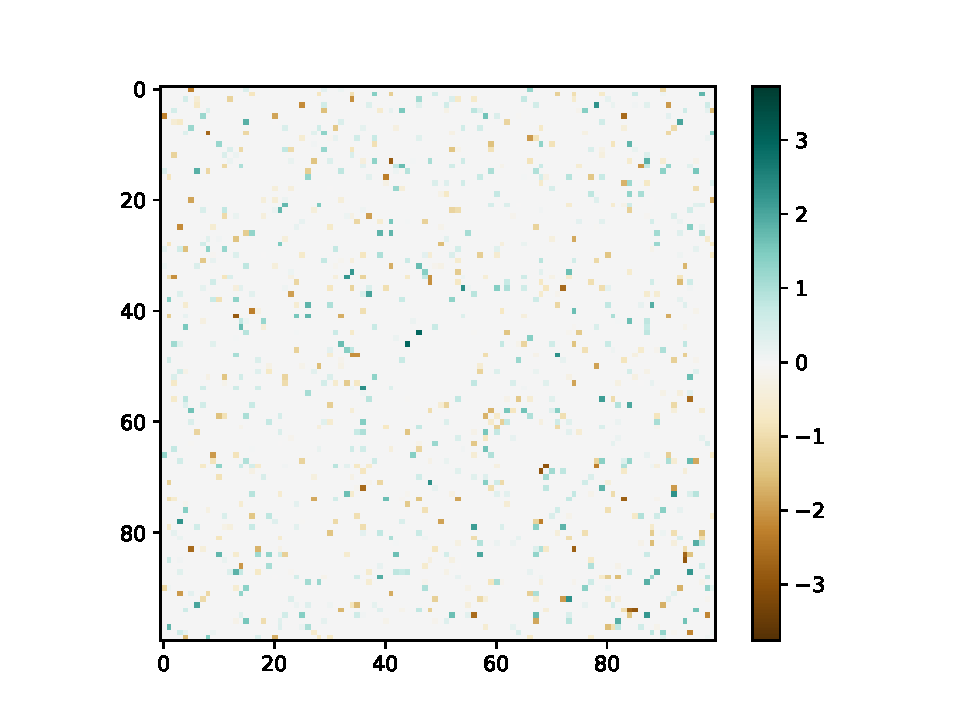
\includegraphics[width=0.7\columnwidth]{Images/Lanczos/A.pdf}
\end{center}
\caption{INSERT CAPTION.}
\label{fig:particle_partition}
\end{figure}

The Lanczos iterations were carried from $k=1$ to $k=n=100$. First, Lanczos was ran without reorthonormalizing the columns of the transform matrix $Q$.


\begin{figure}[t]
\begin{center}
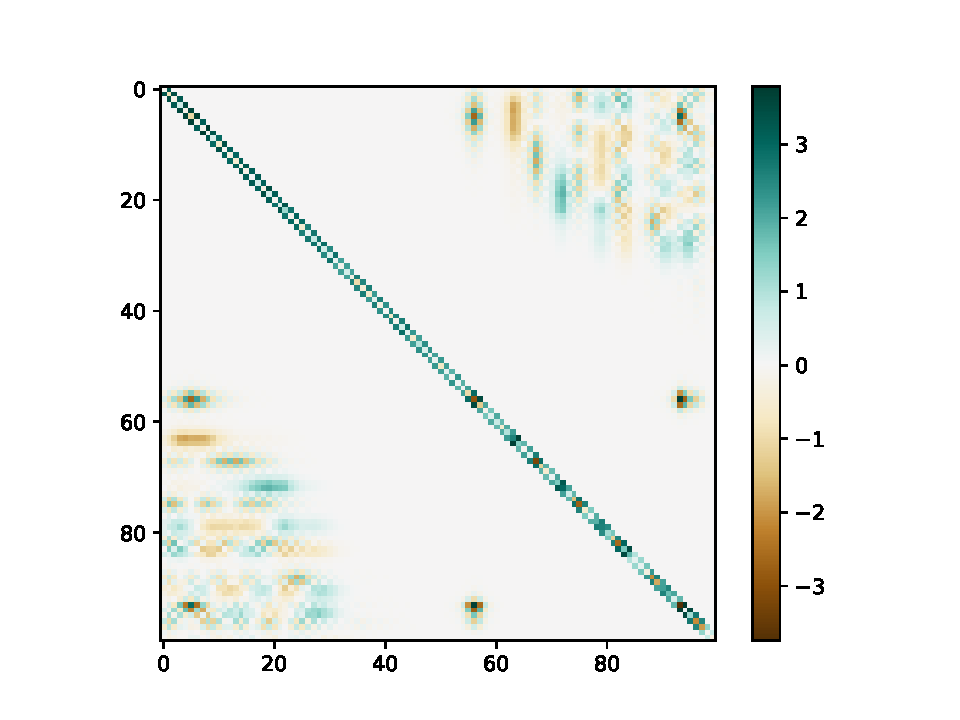
\includegraphics[width=0.7\columnwidth]{Images/Lanczos/T_noReortho.pdf}
\end{center}
\caption{INSERT CAPTION.}
\label{fig:particle_partition}
\end{figure}

Observe how the matrix starts to look tridiagonal, but has some large nonzero entries far away from the diagonal. This is the result of finite precision error. Via the Grahm-Schmidt Procedure, a full reorthonormalization was then done at each Lanczos step. The colormap below shows the result.

\begin{figure}[t]
\begin{center}
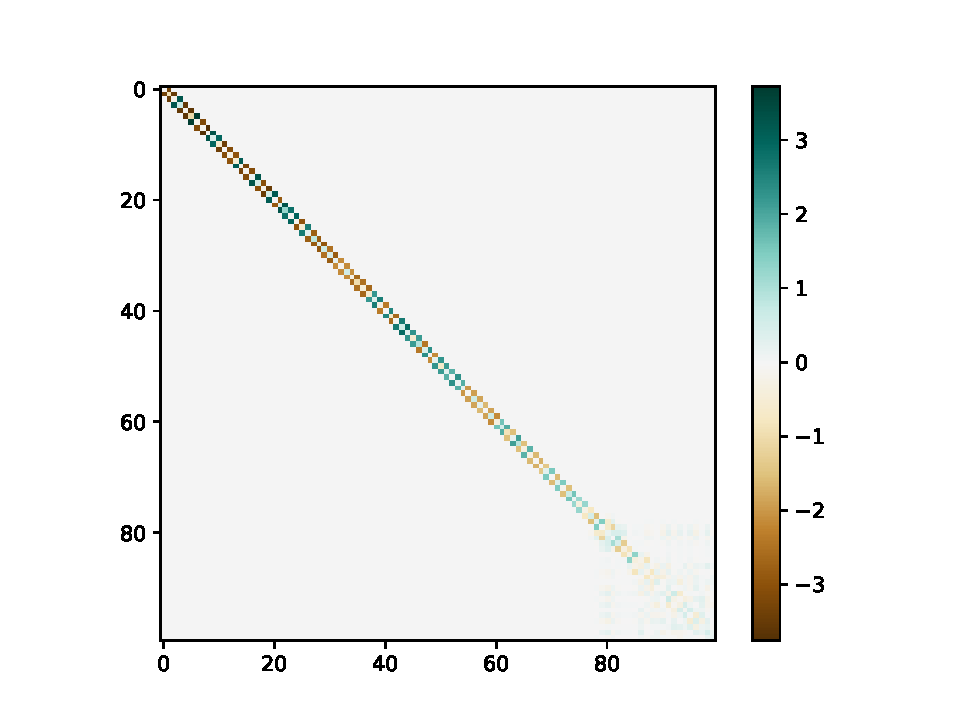
\includegraphics[width=0.7\columnwidth]{Images/Lanczos/T_yesReortho.pdf}
\end{center}
\caption{INSERT CAPTION.}
\label{fig:particle_partition}
\end{figure}

Barring some small nonzero entries in the bottom right, most likely due also to finite precision, the matrix was now tridiagonalized successfully.

The following scatter plot shows the eigenvalues obtained using the Lanczos code linked and those obtained using numpy.linalg.eigsh(). These eigenvalues correspond to the same matrix generated for the plots in the previous section.

\begin{figure}[t]
\begin{center}
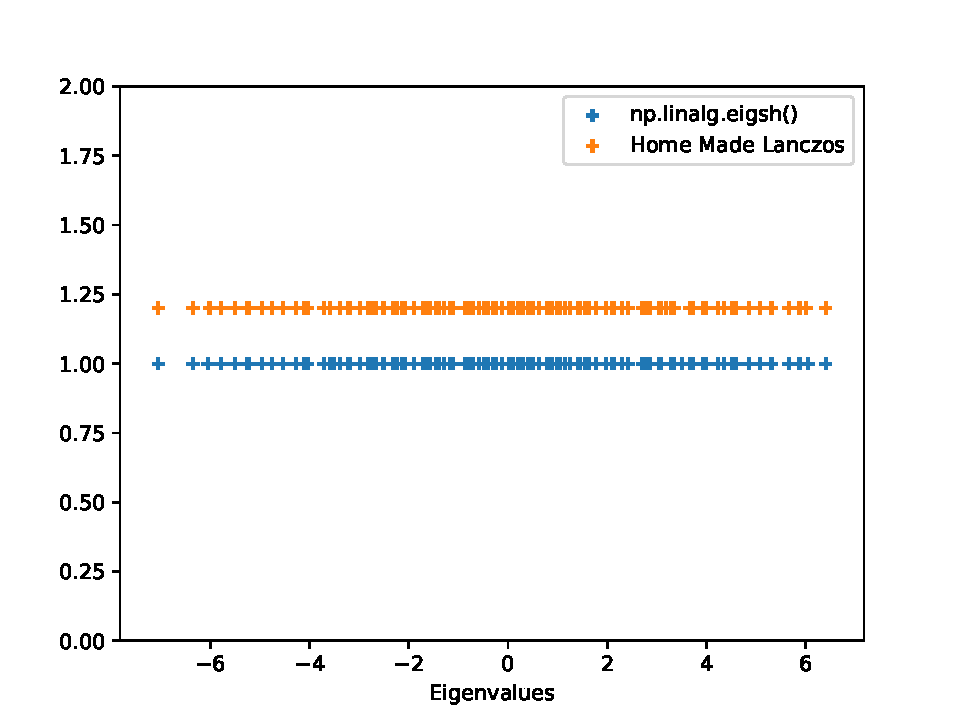
\includegraphics[width=0.7\columnwidth]{Images/Lanczos/eigenvaluesComparison.pdf}
\end{center}
\caption{INSERT CAPTION.}
\label{fig:particle_partition}
\end{figure}